% !TEX TS-program = pdflatex
% !TeX program = pdflatex
% !TEX encoding = UTF-8
% !TEX spellcheck = en_US

\documentclass[xcolor=table]{beamer}

\usepackage{../extra/beamer/karimnlp}

\input{options}

\subtitle[ML for NLP]{Chapter 02\\Machine learning for NLP} 

\changegraphpath{../img/ml4nlp/}

\begin{document}
	

\begin{frame}
	\frametitle{\inserttitle}
	\framesubtitle{ML: Example (Simple Perceptron for binary logical functions)}
	
	\begin{minipage}{0.30\textwidth} 
		\hgraphpage{perceptron.pdf}
	\end{minipage}
	%
	\begin{minipage}{0.59\textwidth}
		\scriptsize
		\begin{itemize}
			\item $ z^{(i)} = x_1^{(i)} w_1 + x_2^{(i)} w_2 + b $
			\item $ \hat{y}^{(i)} = \phi(z^{(i)}) = \begin{cases}
				1 & \text{if } z^{(i)} \ge 0 \\
				0 & \text{otherwise}
			\end{cases} $
			\item $ w_j = w_j + \Delta w_j$ where $ \Delta w_j = \frac{1}{M}\sum_{i=1}^{M} (y^{(i)} - \hat{y}^{(i)}) * x_j^{(i)} $
			\item $ b = b + \Delta b$ where $ \Delta b = \frac{1}{M}\sum_{i=1}^{M} (y^{(i)} - \hat{y}^{(i)})$
		\end{itemize}
	\end{minipage}
	
	\vfill
	
	\begin{exampleblock}{Training a Perceptron for AND function}
		\begin{minipage}{0.2\textwidth} 
			\scriptsize
			\begin{tabular}{|c|c|c|}
				\hline
				x\textsubscript{1} & x\textsubscript{2} & y \\
				\hline
				0 & 0 & 0  \\
				\hline
				0 & 1 & 0 \\
				\hline
				1 & 0 & 0 \\
				\hline
				1 & 1 & 1 \\
				\hline
			\end{tabular}
		\end{minipage}
		%
		\begin{minipage}{0.79\textwidth}
			\scriptsize
			\begin{itemize}
				\item Initially, $ W = [w_1, w_2] = [0, 0]; b = 0 $.
				
				\item It1: $ Z = \hat{Y} = [0, 0, 0, 0] $;
				$ \Delta W = [\frac{1}{4}, \frac{1}{4}], \Delta b = \frac{1}{4} $;
				$ W = [\frac{1}{4}, \frac{1}{4}], b = \frac{1}{4}$.
				
				\item It2: $ Z = [\frac{1}{4}, \frac{2}{4}, \frac{2}{4}, \frac{3}{4}]$; 
				$ \hat{Y} = [1, 1, 1, 1] $;
				$ \Delta W = [\frac{-1}{4}, \frac{-1}{4}], \Delta b = \frac{-3}{4} $;
				$ W = [0, 0], b = \frac{-1}{2} $.
				
				\item It3: $ Z = [\frac{-1}{2}, \frac{-1}{2}, \frac{-1}{2}, \frac{-1}{2}] $; 
				$ \hat{Y} = [1, 1, 1, 1] $; 
				$ \Delta W = [\frac{1}{4}, \frac{1}{4}], \Delta b = \frac{1}{4} $;
				$ W = [\frac{1}{4}, \frac{1}{4}], b = \frac{-1}{4} $.
				
				\item It4: $ Z = [\frac{-1}{4}, 0, 0, \frac{1}{4}] $;
				$ \hat{Y} = Y = [0, 0, 0, 1] $ (STOP)
			\end{itemize}
		\end{minipage}
	\end{exampleblock}
	
\end{frame}
	
\begin{frame}
	\frametitle{\inserttitle}
	\framesubtitle{ML: Algorithms and abbreviations}
	
	\begin{itemize}
		\item Classical Machine Learning Models
		\begin{itemize}
			\item \optword{NB}: Naïve Bayes
			\item \optword{LR}: Logistic Regression
			\item \optword{SVM}: Support Vector Machine
			\item \optword{HMM}: Hidden Markov Model
			\item \optword{MEMM}: Maximum Entropy Markov Model
			\item \optword{CRF}: Conditional Random Fields
		\end{itemize}
		
		\item Neural Network Architectures
		\begin{itemize}
			\item \optword{FFNN}: Feedforward Neural Network
			\begin{itemize}
				\item \optword{MLP}: Multilayer Perceptron
				\item \optword{CNN}: Convolutional Neural Network
			\end{itemize}
			\item \optword{RNN}: Recurrent Neural Network
		\end{itemize}
	\end{itemize}
	
\end{frame}

\begin{frame}
	\frametitle{\inserttitle}
	\framesubtitle{ML: Types of models}
	
	\scriptsize
	\begin{tblr}{
			colspec = {p{.12\textwidth}lp{.37\textwidth}lp{.38\textwidth}},
			row{odd} = {lightblue},
			row{1} = {darkblue, fg=white, font=\bfseries, valign=m, halign=c},
			column{2,4}={white},
			column{1}={bg=darkblue, fg=white, font=\bfseries, valign=m},
			row{even} = {white},
			cell{1}{1}={white},
			colsep=3pt,
			rowsep=3pt,
			stretch = 0,
		}
		
		&& Generative && Discriminative \\
		
		&&&&\\
		
		Text && NB && LR, SVM, MLP, RNN, CNN \\
		
		&&&&\\
		
		Sequence && HMM  && MEMM, CRF, RNN \\
		
	\end{tblr}
	
	\vfill
	
	\begin{itemize}
		\item \optword{Generative models}: learn the joint distribution
		\[
		P(X, Y) = P(Y)P(X \mid Y), \quad
		\hat{Y} = \arg\max_k P(Y_k)P(X \mid Y_k)
		\]
		
		\item \optword{Discriminative models}: learn the conditional distribution
		\[
		\hat{Y} = \arg\max_k P(Y_k \mid X)
		\]
	\end{itemize}
	
\end{frame}


\begin{frame}
	\frametitle{\inserttitle}
	\framesubtitle{NLP: Text classification}
	
	\begin{itemize}
		\item Document-level classification:
		\begin{itemize}
			\item \optword{Sentiment analysis}: classifying text into positive, negative, or neutral sentiment.
			\item \optword{Spam detection}: classifying a message as spam or not spam.
			\item \optword{Figurative language detection}: classifying text as metaphorical, ironic, etc.
		\end{itemize}
		
		\item Sentence-level classification:
		\begin{itemize}
			\item \optword{Extractive summarization}: classifying sentences as belonging to the summary or not.
			\item \optword{Textual entailment (NLI)}: determining whether one sentence entails another.
		\end{itemize}
	\end{itemize}
	
\end{frame}


\begin{frame}
	\frametitle{\inserttitle}
	\framesubtitle{NLP: Sequence labeling}
	
	\begin{itemize}
		\item Given a sentence, a label is assigned to each word.
		
		\item Example: \expword{Assigning a part-of-speech to each word}.
		
		\item The class of a word may depend on preceding and/or following words.
		
		\item \textbf{Problem}: how to assign labels to contiguous sequences of words (multi-token entities)?
		
		\item Example: \expword{[\textit{Abdelkrime Aries}]\textsubscript{\bfseries PERSON} is a teacher at the [\textit{Ecole nationale Supérieure d'Informatique}]\textsubscript{\bfseries INSTITUTE}}
	\end{itemize}
	
\end{frame}


\begin{frame}
	\frametitle{\insertshortsubtitle: \insertsection}
	\framesubtitle{NLP: Sequence classification (BIO representation)}
	
	\begin{itemize}
		\item \keyword{BIO}: Beginning, Inside, Outside
		
		\item For each class \textbf{CLS}, two labels are defined: \textbf{B-CLS} and \textbf{I-CLS}.
		
		\item \optword{B-CLS} marks the beginning of an entity.
		
		\item \optword{I-CLS} marks the continuation of the same entity.
		
		\item \optword{O} indicates that the token does not belong to any class.
		
		\item Ensures correct identification of boundaries between adjacent entities.
		
		\item Example: \expword{Abdelkrime/\textsubscript{\bfseries B-PERSON} Aries/\textsubscript{\bfseries I-PERSON} is/\textsubscript{\bfseries O} a/\textsubscript{\bfseries O} teacher/\textsubscript{\bfseries O} at/\textsubscript{\bfseries O} the/\textsubscript{\bfseries O} Ecole/\textsubscript{\bfseries B-INSTITUTE} nationale/\textsubscript{\bfseries I-INSTITUTE} Supérieure/\textsubscript{\bfseries I-INSTITUTE} d'/\textsubscript{\bfseries I-INSTITUTE} Informatique/\textsubscript{\bfseries I-INSTITUTE}}
	\end{itemize}
\end{frame}


\begin{frame}
	\frametitle{\inserttitle}
	\framesubtitle{NLP: Text generation}
	
	\begin{itemize}
		\item Text generation is the task of generating a sequence of tokens by modeling conditional probabilities over a vocabulary.
	\end{itemize}
	
	\[
	\hat{w}_i = \arg\max_{w_i} P(w_i \mid \hat{w}_1, \dots, \hat{w}_{i-1})
	\]
	
\end{frame}


\begin{frame}
	\frametitle{\inserttitle}
	\framesubtitle{\insertshortsubtitle: Plan}
	
	\begin{multicols}{2}
		\small
		\tableofcontents
	\end{multicols}
\end{frame}



%===================================================================================
\section{Traditional ML and MLP-based architectures}
%===================================================================================

\begin{frame}
	\frametitle{\insertshortsubtitle}
	\framesubtitle{\insertsection}
	
	\begin{itemize}
		\item Text classification requires a fixed-size representation of each text (i.e., a vector).
		
		\item Sequence labeling:
		\begin{itemize}
			\item Hidden Markov Models (HMMs) have been traditionally used.
			\item MLPs and other models can be applied using a fixed-size context window, approximating Markov assumptions.
		\end{itemize}
		
		\item Text generation:
		\begin{itemize}
			\item n-gram language models (e.g., bigrams) have been traditionally used.
			\item MLPs and other models can also be applied using fixed-size context windows.
		\end{itemize}
	\end{itemize}
	
\end{frame}


\subsection{Text classification}

\begin{frame}
	\frametitle{\insertshortsubtitle: \insertsection}
	\framesubtitle{\insertsubsection: Examples}
	
	\vgraphpage{text_class_trad_exp.pdf}
	
\end{frame}

\subsection{Sequence labeling}


\begin{frame}
	\frametitle{\insertshortsubtitle: \insertsection}
	\framesubtitle{\insertsubsection: Markov model}
	
	\begin{minipage}{.64\textwidth}
			\begin{itemize}
					\item Markov hypothesis
					\item $ P(q_i = a | q_1, \ldots, q_{i-1}) \approx P(q_i = a | q_{i-1}) $
					\item $Q = \{q_1, q_2, \ldots, q_n\}$: stats.
					\item $A = \begin{bmatrix}%
							a_{11} & a_{12} & \ldots & a_{1n} \\
							a_{21} & a_{22} & \ldots & a_{2n} \\
							\vdots & \vdots & \ddots & \vdots \\
							a_{n1} & a_{n2} & \ldots & a_{nn} \\
						\end{bmatrix}$: transition probability matrix.
					\item $\sum_j a_{ij} = 1,\, \forall i$.
				\end{itemize}
		\end{minipage}
	\begin{minipage}{.35\textwidth}
			\hspace*{-1cm}
			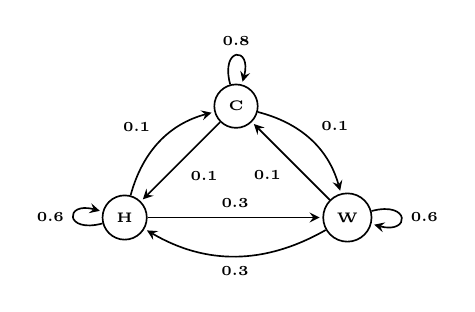
\begin{tikzpicture}[
					> = stealth, % arrow head style
					shorten > = 1pt, % don't touch arrow head to node
					auto,
					node distance = 2cm, % distance between nodes
					semithick, % line style
					font=\tiny\bfseries
					]
					
					\node[circle,draw] (qC) {C};
					\node[circle,draw] (qH) [below left of=qC] {H};
					\node[circle,draw] (qW) [below right of=qC] {W};
					
					\path[->] 	
					(qC) 	edge [loop above] node {0.8} ()
					edge [] node {0.1} (qH)
					edge [bend left] node {0.1} (qW)
					(qH) 	edge [loop left] node {0.6} ()
					edge [bend left] node {0.1} (qC)
					edge [] node {0.3} (qW)
					(qW)	edge [loop right] node {0.6} ()
					edge [bend left] node {0.3} (qH)
					edge [] node {0.1} (qC);
				\end{tikzpicture}
		\end{minipage}
	
	\begin{itemize}
			\item $\pi = [\pi_1, \pi_2, \ldots, \pi_n ]$: states initial probability distribution.
			\item $\sum_i \pi_i = 1$.
			\vspace{-6pt}\item E.g. \expword{Calculate $P(H\, W\, C\, C)$ where $\pi = [\overbrace{0.1}^C, \overbrace{0.7}^H, \overbrace{0.2}^W]$}.
		\end{itemize}
\end{frame}

\begin{frame}
	\frametitle{\insertshortsubtitle: \insertsection}
	\framesubtitle{\insertsubsection: Hidden Markov model}
	\begin{minipage}{.54\textwidth}
			\begin{itemize}
					\item $Q = \{q_1, q_2, \ldots, q_n\}$: states.
					\item $A$: transition probability matrix where $\sum_j a_{ij} = 1,\, \forall i$.
					\item $O = o_1 o_2 \ldots o_T$: sequence of observed events (words).
					\item $B = b_i(o_t)$: observation probabilities (\keyword{emission probabilities}), each represents the probability of generating an observation $o_t$ in a state $q_i$.
				\end{itemize}
		\end{minipage}
	\begin{minipage}{.45\textwidth}
			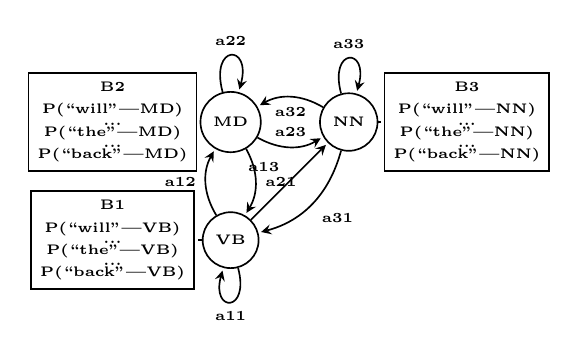
\begin{tikzpicture}[
					> = stealth, % arrow head style
					shorten > = 1pt, % don't touch arrow head to node
					auto,
					node distance = 1.5cm, % distance between nodes
					semithick, % line style
					font=\bfseries\fontsize{4}{4}\selectfont
					]
					
					\node[circle,draw] (q2) {MD};
					\node[align=center,draw] (q2e) [left of=q2] {B2\\ \\P(``will"|MD)\\...\\P(``the"|MD)\\...\\P(``back"|MD)};
					\node[circle,draw] (q3) [right of=q2] {NN};
					\node[align=center,draw] (q3e) [right of=q3] {B3\\ \\P(``will"|NN)\\...\\P(``the"|NN)\\...\\P(``back"|NN)};
					\node[circle,draw] (q1) [below of=q2] {VB};
					\node[align=center,draw] (q1e) [left of=q1] {B1\\ \\P(``will"|VB)\\...\\P(``the"|VB)\\...\\P(``back"|VB)};
					
					\path[->] 	
					(q1) 	edge [loop below] node {a11} ()
					edge [bend left] node {a12} (q2)
					edge [] node {a13} (q3)
					(q2) 	edge [loop above] node {a22} ()
					edge [bend left] node {a21} (q1)
					edge [bend right] node {a23} (q3)
					(q3)	edge [loop above] node {a33} ()
					edge [bend left] node {a31} (q1)
					edge [bend right] node {a32} (q2);
					
					\path[dashed] 	
					(q1) 	edge [] node {} (q1e)
					(q2) 	edge [] node {} (q2e)
					(q3) 	edge [] node {} (q3e);
					
				\end{tikzpicture}
		\end{minipage}
	
	\begin{itemize}
			\item $\pi = [\pi_1, \pi_2, \ldots, \pi_n ]$: states initial probability distribution.
			\item $\sum_i \pi_i = 1$.
		\end{itemize}
	
\end{frame}

\begin{frame}
	\frametitle{\insertshortsubtitle: \insertsection}
	\framesubtitle{\insertsubsection: HMM Training}
	
	\begin{itemize}
			\item States correspond to tags (categories) $t_i$.
			\item We define a special start-of-sentence tag \keyword{START}.
			\item Observations $o_i$ correspond to words $w_i$.
			\item \keyword{C}: frequency (count) in the training corpus.
			
		\end{itemize}
	
	\begin{block}{HMM training}
			\[
			\text{Transition probabilities: } P(t_i | t_{i-1}) = \frac{C(t_{i-1}, t_i)}{C(t_{i-1})} 
			\]\[
			\text{Emission probabilities: } P(w_i | t_i) = \frac{C(t_i, w_i)}{C(t_i)}
			\]\[
			\text{Initial distribution: } \pi_i = P(t_i | START) = \frac{C(START, t_i)}{C(START)}
			\]
		\end{block}
\end{frame}

\begin{frame}
	\frametitle{\insertshortsubtitle: \insertsection}
	\framesubtitle{\insertsubsection: HMM Labeling (tag decoding)}
	
	\begin{itemize}
			\item Given
			\begin{itemize}
				\item a Hidden Markov Model $\lambda = (A, B, \pi)$,
				\item a sequence of observations $w = w_1 w_2 \ldots w_n$,
				\item $t_0 = START$
			\end{itemize}
			\item Estimate a sequence of labels $\hat{t} = \hat{t}_1 \hat{t}_2 \ldots \hat{t}_n$
		\end{itemize}
	
	\begin{block}{Labels' decoding using HMM}
			\[
			\hat{t} = \arg\max\limits_t P(t | w) = \arg\max\limits_t \frac{P(w|t) P(t)}{P(w)} = \arg\max\limits_t P(w|t) P(t)%\text{ tel que } t = t_1 t_2 \ldots t_n
			\]
			
			\[ 
			P(w | t) = \prod\limits_{i=1}^n P(w_i|t_i) 
			\hskip2cm
			P(t) = \prod\limits_{i=1}^n P(t_i|t_{i-1}) 
			\]
			
			\[
			\hat{t} = \arg\max\limits_t \prod\limits_{i=1}^n P(w_i|t_i) P(t_i|t_{i-1})
			\]
		\end{block}
\end{frame}

\begin{frame}
	\frametitle{\insertshortsubtitle: \insertsection}
	\framesubtitle{\insertsubsection: HMM \& Viterbi algorithm}
	
	\begin{block}{Viterbi}
			\scriptsize
			\begin{algorithm}[H]
		%				\vskip-1em
					\KwData{$w = w_1 \ldots w_T$, HMM $\lambda = (A, B, \pi)$ with $N$ states}
					\KwResult{$best\_path$, $prob\_path$}
					
					Create a matrix $viterbi[N, T]$\;
					
					\lForEach{state $ s = 1 \ldots N$}{
							$viterbi[s, 1] = \pi_s * b_s(w_1);\, backpointer[s, 1] = 0$
						}
					
					\ForEach{tag $ t = 2 \ldots T$}{
							\ForEach{state $ s = 1 \ldots N$}{
									$viterbi[s, t] = \max\limits_{s'=1}^N viterbi[s', t-1] * a_{s',s} * b_s(w_t)$\;
									$backpointer[s, t] = \arg\max\limits_{s'=1}^N viterbi[s', t-1] * a_{s',s} * b_s(w_t)$\;
								}
						}
					
					$prob\_path = \max\limits_{s=1}^N viterbi[s, T];\, pointer\_path = \arg\max\limits_{s=1}^N viterbi[s, T]$\;
					
					$best\_path$ is the path starting from $pointer\_path$ and following $backpointer$
					
					\Return $best\_path$, $prob\_path$\;
					
				\end{algorithm}
		\end{block}
	
\end{frame}

\begin{frame}
	\frametitle{\insertshortsubtitle: \insertsection}
	\framesubtitle{\insertsubsection: MEMM/MLP}
	
	\begin{itemize}
			\item Let $x_{n}^{m} = x_n x_{n+1} \ldots x_{m-1} x_m$ denote a subsequence.
			\item Given 
			\begin{itemize}
				\item a sequence of observations $w = w_1 w_2 \ldots w_n$,
				\item a set of feature functions $f_j$ defined on the sequence (e.g., whether a word is capitalized),
			\end{itemize}
			\item Estimate a sequence of tags $\hat{t} = \hat{t}_1 \hat{t}_2 \ldots \hat{t}_n$
		\end{itemize}
	
	\begin{block}{Decoding with MEMM}
			\[
			\hat{t} = \arg\max_t P(t | w) = \arg\max_{t} \prod_{i=1}^{n} P(t_i \mid w_{i-l}^{i+l}, t_{i-k}^{i-1})
			\]
			
			\[
			\hat{t} = \arg\max\limits_t \prod\limits_{i}  
			\frac{exp\left(\sum_j \theta_j f_j(t_i, w_{i-l}^{i+l}, t_{i-k}^{i-1})\right)}%
			{\sum_{t' \in tags} exp\left(\sum_j \theta_j f_j(t'_i, w_{i-l}^{i+l}, t_{i-k}^{i-1})\right)}
			\]
		\end{block}
	
\end{frame}


\subsection{Text generation}

\begin{frame}
	\frametitle{\insertshortsubtitle: \insertsection}
	\framesubtitle{\insertsubsection}
	
	\begin{itemize}
		\item Using n-grams of size \(n\),
		\item The probability of a word \(w_i\) is conditioned on the preceding \(n-1\) words.
		\item The predicted word is the one with the highest conditional probability:
		\[
		\hat{w}_i = \arg\max\limits_{w_i} P(w_i \mid w_{i-n+1}, \dots, w_{i-1})
		\]
		\item N-gram probabilities are estimated from a training corpus.
		\item This topic will be discussed in the \keyword{``Language Models''} chapter.
		\item Multi-Layer Perceptrons (MLPs) can also model word probabilities using a fixed-size context window, analogous to n-grams.
	\end{itemize}
	
\end{frame}

\begin{frame}
	\frametitle{\insertshortsubtitle: \insertsection}
	\framesubtitle{\insertsubsection: MLP-based text generation (Example)}
	
	\[\hat{w}_i = \arg\max\limits_{w_i} P(w_i | \hat{w}_{i-N+1}, \cdots, \hat{w}_{i-1})\]
	
	\begin{center}
		\vgraphpage[0.7\textheight]{text_gen_MLP_exp.pdf}
	\end{center}
	
\end{frame}

\subsection{Embedding layer}

\begin{frame}
	\frametitle{\insertshortsubtitle: \insertsection}
	\framesubtitle{\insertsubsection}
	
%	\[\hat{w}_i = \arg\max\limits_{w_i} P(w_i | \hat{w}_{i-N+1}, \cdots, \hat{w}_{i-1})\]
	
%	\begin{center}
%		\vgraphpage[0.7\textheight]{text_emb_exp.pdf}
%	\end{center}
	\hgraphpage[\textwidth]{text_emb_exp.pdf}
	
\end{frame}


%===================================================================================
\section{CNN-based architectures}
%===================================================================================

\begin{frame}
	\frametitle{\insertshortsubtitle}
	\framesubtitle{\insertsection}
	
	\begin{itemize}
		\item Text classification:
		\begin{itemize}
			\item Requires a fixed-size representation for all texts (e.g., embedding matrix).
			\item A fully connected layer (MLP) is used to produce class probabilities.
		\end{itemize}
		
		\item Sequence labeling:
		\begin{itemize}
			\item Similar to text classification, but previous predicted tags can be incorporated as an additional input channel to capture label dependencies.
		\end{itemize}
		
		\item Text generation:
		\begin{itemize}
			\item Similar to classification; instead of predicting a class, the model predicts the next word in the sequence, typically using a softmax over the vocabulary.
		\end{itemize}
	\end{itemize}
	
\end{frame}

\subsection{Text classification}

\begin{frame}
	\frametitle{\insertshortsubtitle: \insertsection}
	\framesubtitle{\insertsubsection}
	
	\begin{itemize}
		\item Each word in the text is represented by a vector of dimension $N$ (word embedding).
		\item Word vectors are stacked to form a matrix of size $M \times N$, where $M$ is the number of words.
		\item A one-dimensional convolution with a filter of size $K \times N$ is applied (covering $K$ words at a time).
		\item Several filters can be used to learn multiple representations.
		\item Pooling (e.g., max-pooling) can also be applied.
		\item A fully connected layer (MLP) is used at the end to predict the class.
		\item \textbf{Problem}: Neural networks require a fixed-size input; variable-length texts cannot be processed directly.
		\item \textbf{Solution}: \textcolor{yellow!30}{Define a maximum sequence length: pad shorter texts with zeros and truncate longer texts.}
	\end{itemize}
	
\end{frame}

\begin{frame}
	\frametitle{\insertshortsubtitle: \insertsection}
	\framesubtitle{\insertsubsection: Examples}
	
	\vgraphpage{text_class_CNN_exp.pdf}
	
\end{frame}

\subsection{Sequence labeling}

\begin{frame}
	\frametitle{\insertshortsubtitle: \insertsection}
	\framesubtitle{\insertsubsection}
	
	\vgraphpage{text_seq_CNN_exp.pdf}
	
\end{frame}


\subsection{Text generation}

\begin{frame}
	\frametitle{\insertshortsubtitle: \insertsection}
	\framesubtitle{\insertsubsection}
	
	\vgraphpage{text_gen_CNN_exp.pdf}
	
\end{frame}


%===================================================================================
\section{RNN-based architectures}
%===================================================================================

\begin{frame}
	\frametitle{\insertshortsubtitle}
	\framesubtitle{\insertsection}
	
	\begin{itemize}
		\item Text classification:
		\begin{itemize}
			\item The final hidden state of the RNN is fed into a fully connected layer (MLP).
			\item The MLP predicts the class label.
		\end{itemize}
		
		\item Sequence tagging:
		\begin{itemize}
			\item Each hidden state produced by the RNN is passed through a fully connected layer (MLP) to predict the corresponding label.
		\end{itemize}
		
		\item Text generation:
		\begin{itemize}
			\item The model predicts the next word at each time step until an end-of-sentence token is generated.
		\end{itemize}
	\end{itemize}
	
	
\end{frame}

\subsection{Text classification}

\begin{frame}
	\frametitle{\insertshortsubtitle: \insertsection}
	\framesubtitle{\insertsubsection}
	
	\begin{itemize}
		\item Each word in the text is represented by a vector of dimension $N$ (word embedding).
		\item The RNN processes the sequence of $M$ words, producing $M$ hidden states (one per word).
		\item Each cell computes a hidden state that is passed to the next time step.
		\item The last hidden state summarizes the entire text and is fed into a fully connected layer (MLP) to predict the text's class.
		\item \textbf{Problem}: Neural networks require fixed-size inputs; sequences of different lengths cannot be processed directly.
		\item \textbf{Solution}: \textcolor{yellow!30}{Define a maximum sequence length: pad shorter texts and truncate longer ones.}
	\end{itemize}
	
	
\end{frame}

\begin{frame}
	\frametitle{\insertshortsubtitle: \insertsection}
	\framesubtitle{\insertsubsection: Example}
	
	\vgraphpage{text_class_RNN_exp.pdf}
	
\end{frame}


\subsection{Sequence labeling}

\begin{frame}
	\frametitle{\insertshortsubtitle: \insertsection}
	\framesubtitle{\insertsubsection: Example}
	
	\vgraphpage{seq_class_RNN_exp.pdf}
	
\end{frame}


\subsection{Text generation}

\begin{frame}
	\frametitle{\insertshortsubtitle: \insertsection}
	\framesubtitle{\insertsubsection: Language model}
	
	\vgraphpage{text_gen_RNN_exp.pdf}
	
\end{frame}

\begin{frame}
	\frametitle{\insertshortsubtitle: \insertsection}
	\framesubtitle{\insertsubsection: GAN-based decoder}
	
	\begin{figure}
		\hgraphpage{text_gen_RNNGAN_exp_.pdf}
		\caption{The illustration of SeqGAN. 
			Left: \textit{D} is trained over the real data and the generated data by \textit{G}. 
			Right: \textit{G} is trained by policy gradient where the final reward signal is provided
			by \textit{D} and is passed back to the intermediate action value via Monte Carlo search. \cite{SeqGAN}}
	\end{figure}
	
\end{frame}


%===================================================================================
\section{Transformer-based architectures}
%===================================================================================


\begin{frame}
	\frametitle{\insertshortsubtitle}
	\framesubtitle{\insertsection}
	
	\begin{itemize}
		\item Transformers can be applied to the three main NLP tasks:
		\begin{itemize}
			\item Both encoder-only and encoder-decoder architectures can be used for text classification.
			\item Encoder-only architectures are better suited for sequence labeling/classification tasks.
			\item Decoder-only architectures are better suited for text generation tasks.
		\end{itemize}
	\end{itemize}
	
	
\end{frame}


\subsection{Text classification}

\begin{frame}
	\frametitle{\insertshortsubtitle: \insertsection}
	\framesubtitle{\insertsubsection: Encoder-based (Example)}
	
	\begin{center}
		\vgraphpage{text_class_bert_exp.pdf}
	\end{center}
	
\end{frame}

\begin{frame}
	\frametitle{\insertshortsubtitle: \insertsection}
	\framesubtitle{\insertsubsection: Decoder-based (Example)}
	
	\hgraphpage{gpt-arch_.pdf}
	
\end{frame}

\begin{frame}
	\frametitle{\insertshortsubtitle: \insertsection}
	\framesubtitle{\insertsubsection: Full-transformer (Example)}
	
	\hgraphpage{t5-arch_.pdf}
	
\end{frame}


\subsection{Sequence labeling}

\begin{frame}
	\frametitle{\insertshortsubtitle: \insertsection}
	\framesubtitle{\insertsubsection: Encoder-based (Example)}
	
	\begin{center}
		\vgraphpage{text_seq_bert_exp.pdf}
	\end{center}
	
\end{frame}

\begin{frame}
	\frametitle{\insertshortsubtitle: \insertsection}
	\framesubtitle{\insertsubsection: Decoder-based and Full-transformer}
	
	\begin{itemize}
		\item Conceptual ideas (not derived from published research):
		\item Sequence tagging can be formulated as generating tags one by one (autoregressive).
		\item For full (encoder-decoder) transformers:
		\begin{itemize}
			\item The encoder receives the sentence as input.
			\item The decoder receives the previously predicted tags and attends to the encoder outputs to predict the next tag.
		\end{itemize}
		\item For decoder-only architectures:
		\begin{itemize}
			\item The decoder receives a concatenation of the sentence and previously predicted tags.
			\item An optional separator token can distinguish sentence tokens from tag tokens.
		\end{itemize}
	\end{itemize}
	
	
\end{frame}


\subsection{Text generation}

\begin{frame}
	\frametitle{\insertshortsubtitle: \insertsection}
	\framesubtitle{\insertsubsection}
	
	\begin{itemize}
		\item Decoder-only language models are naturally suited for autoregressive text generation.
		\item Encoder-only language models:
		\begin{itemize}
			\item Use Masked Language Modeling (MLM) for tasks such as text infilling.
			\item Their outputs can be fed into a separate decoder to generate sequences.
			\item Other generation approaches are also possible based on encoder representations.
		\end{itemize}
	\end{itemize}
	
	
\end{frame}



\insertbibliography{NLP02}{*}
	
\end{document}

